\documentclass[a4paper]{jpconf}
\usepackage{graphicx}
\usepackage{subfig}
\begin{document}
\title{von Neumann - Wigner Darboux deformed truncated oscillator.} 

\author{L\' opez Mej\' ia L and Fern\' andez-Garc\' ia N}

\address{Instituto Polit\' ecnico Nacional, UPIITA, Av. I.P.N. 2580, Col. La Laguna Ticom\' an, 07360 M\' exico
City, Mexico.}

\ead{llopezm1808@alumno.ipn.mx}

\begin{abstract}
Starting from a radial truncated harmonic oscillator with zero angular momentum, the well known Darboux transformation is used for constructing a von Neumann - Wigner potential type. The method consists in using as a feed function one solution in the continuous regime for implementing a degenerated version of the second order Darboux transformation. After the continuity of the solutions is guaranteed, it is shown that the resulting system, in addition to the scattering and conventional bound states, contains a square integrable wave function associated to one energy eigenvalue belonging to the continuous part of the spectrum, which is justly the eigenvalue corresponding to the transformation function. 



\end{abstract}
%%%%%%%%%%%%%%%%%%%%%%%%%%%%%%%%%%%%%%%%%%%%%%%%%%%%%%%%%%%%%%%%%%%%%%%%%%%%%%%%%
\section{Introduction.}
%%%%%%%%%%%%%%%%%%%%%%%%%%%%%%%%%%%%%%%%%%%%%%%%%%%%%%%%%%%%%%%%%%%%%%%%%%%%%%%%% 

In 1929, von Neumann and Wigner proposed a method to construct a potential that could admit a square integrable solution in the continuous spectrum regime \cite{vNW}; nevertheless, the resulting potential has an oscillatory behavior that goes to zero as $1/r$, which, in principle, does not have a direct correspondence with the behavior of any physical system. In addition, the method has the limitation that only the solution corresponding to the bound state in the continuum can be analytically known, the rest of the solutions would have to be obtained by directly solving the Schr\" odinger equation. For that reasons, at those times, these kind of potentials were considered simply as toy models that could not  occur in nature. However, according to a relatively recent works, the possible existence of such systems has been explored with new techniques in a lot of classical and quantum contexts that involves waves propagation or even in the growing of semiconductor heterostructures by molecular bean epitaxy \cite{Stillinger,Anzor,Stahlhofen,Nature,Pappademos,Mondragon,Nico1,Nico2,Capasso}.\\
The Darboux transformation, also known in the quantum mechanics context as factorization method or supersymmetric quantum mechanics, is a powerful mathematical tool for constructing solutions of the Schr\" odinger equation starting from a system whose solution is known \cite{Witten,Mielnik,Darboux}. This transformation has been widely used in quantum mechanics for constructing isospectral or quasi-isospectral Hamiltonians of well known systems like harmonic oscillator, the hydrogen atom, to name a few (see for example \cite{David,Oscar} and references therein), it has even been used to construct non-Hermitian Hamiltonians with a purely real spectrum \cite{Zurika,Nico3}.\\
In this work, a degenerated version of the  second order Darboux transformation is implemented on the truncated radial harmonic oscillator with zero angular momentum for constructing a von Neumann - Winger type potential.  The scattering and bound states of the deformed system are obtained and the condition for the existence of the bound state in the continuum is established.\\
In section 2 we present a short description of the von Neumann - Wigner method for constructing bound states in the continuum. Section 3 presents how the Darboux transformation operates. In section 4 the general solution for the truncated radial oscillator is presented. In sections 5 and 6 the degenerated version of the Darboux transformation is used for deforming the starting system (truncated radial harmonic oscillator) and the condition for the existence of the bound state in the continuum is stablished. Finally, in section 6, we finish the paper with some concluding remarks.

%%%%%%%%%%%%%%%%%%%%%%%%%%%%%%%%%%%%%%%%%%%%%%%%%%%%%%%%%%%%%%%%%%%%%%%%%%%%%%%%%
\section{The von Neumann - Wigner type potentials.}
%%%%%%%%%%%%%%%%%%%%%%%%%%%%%%%%%%%%%%%%%%%%%%%%%%%%%%%%%%%%%%%%%%%%%%%%%%%%%%%%%


In 1929, unlike what is usually done, von Neumann and Wigner investigated an alternative mechanism to obtain information from the stationary Schr\" odinger equation \cite{vNW,Stillinger}: instead of introducing an interaction potential and  looking for the corresponding eigenvalues and eigenfunctions, they proposed the existence of a square integrable solution associated with an eigenvalue in the continuous regime,  such that the task was to find the kind of potentials which fulfills that property. Bellow, a brief description of the method is presented.\\
Let us write the stationary radial Schr\" odinger equation as follows (in appropriate units and with angular momentum $l=0$):

\begin{equation}
V(r)=E+\frac{1}{2}\frac{\nabla^2\psi(r)}{\psi(r)}.\label{vNW-V0}
\end{equation}

The main idea of the method is to assume the existence of a solution which can be written as the product of a free particle solution and a modulation function $f(r)$, that is, 

\begin{equation}
\psi(r)=f(r)\,\frac{\sin{kr}}{kr},\label{vNW-Psi0}
\end{equation}
with $E=k^2$. The substitution of (\ref{vNW-Psi0}) into (\ref{vNW-V0}) leads to the next expression for the potential in terms of $f(r)$ 

\begin{equation}
V(r)= k \cot{kr}\,\frac{f'(r)}{f(r)}+\frac{1}{2}\frac{f''(r)}{f(r)}, \quad {\rm where}\quad '\equiv \frac{d}{dr}.\label{vNW-V1}
\end{equation}

So we have to look for an appropriate function $f(r)$ that, on the one hand, guarantees that the potential is free of singularities and, on the other, the wave function $\psi(r)$ (associated with the eigenvalue $E=k^2$) is square integrable.
In order to obtain a potential free of singularities, the zeros of $f(r)$ and the product $f(r) \sin{kr}$ must be compensated with zeros, at least of the same order, of $f''(r)$ and $f'(r)$, respectively. With this in mind, von Neumann and Wigner founded the next form for the modulation function \cite{vNW}:

\begin{equation}
f(r)=\frac{1}{A^2+[2kr-\sin{2kr}]^2},\label{vNW-f}
\end{equation}


\begin{figure}
\begin{center}
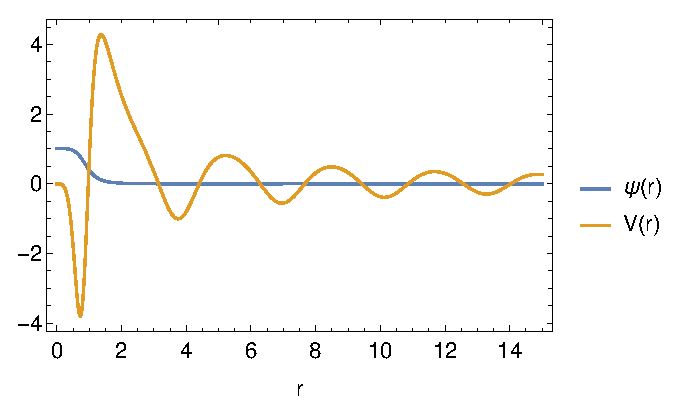
\includegraphics[scale=0.7]{vNW-Figure.eps}
\end{center}
\caption{\label{vNW-Figure} The von Neumann - Wigner potential (dashed line) and the corresponding bound state in the continuum (solid line) for $k=1$ and $A=1$.}
\end{figure}
where A is a nonzero real constant. The Figure \ref{vNW-Figure} shows the von Neumann - Wigner potential and its corresponding bound state in the continuum for $E=k^2=1$ and the parameter $A=1$, which are obtained substituting the function $f(r)$ into (\ref{vNW-Psi0}) and (\ref{vNW-V1}). The possibilities for the function $f(r)$ are not limited to that presented by von Neumann and Wigner (see for example \cite{Stillinger}), but all of them have an asymptotic oscillatory behavior given by \cite{Stahlhofen}:

\begin{equation}
\lim_{r\rightarrow\infty}V(r) \rightarrow a\,\frac{\sin{br}}{r}+ O\left(\frac{1}{r^2}\right).\label{vNW-V2}
\end{equation}
If $|b| <|a|$, the bound state in the continuum (BIC) appears for the energy eigenvalue $E=b^2/4$, that is, the BIC appears for a very specific value of the energy, which is determined by the oscillatory frequency of the potential. The physical interpretation of this phenomenon is that it appears as a result of the destructive interference caused by the multiple crests of the potential.\\
The peculiar behavior of the von Neumann - Wigner potentials meant that, at the time they were proposed, they were considered simply as toy models that could not be present in nature. However, there are recent works that suggest BICs may appear in material systems as dielectric photonic crystals, optical waveguides and fibres, quantum dots,
graphene and topological insulators (see \cite{Nature} and references cited there). The construction of von Neumann-Wigner  potentials, in addition to be considered toy models, have the problem that only one solution to the Schr\" odinger equation is known, which is precisely the bound state in the continuum. Therefore, new mechanisms, based on the supersymmetric quantum mechanics or Darboux transformation, have been created to generate this type of potentials \cite{Pappademos,Mondragon,Nico1,Nico2}. In the next section we will present the mechanism of the degenerated Darboux transformation, which will be used for constructing a von Neumann - Wigner Darboux deformed truncated oscillator.

%%%%%%%%%%%%%%%%%%%%%%%%%%%%%%%%%%%%%%%%%%%%%%%%%%%%%%%%%%%%%%%%%%%%%%%%%%%%%%%%%
\section{Degenerated Darboux transformation.}
%%%%%%%%%%%%%%%%%%%%%%%%%%%%%%%%%%%%%%%%%%%%%%%%%%%%%%%%%%%%%%%%%%%%%%%%%%%%%%%%%

The Darboux transformation is a mathematical tool widely used for finding solutions to differential equations from a starting one, whose solution is completely known \cite{Nico3,Springer,Nico4}. To establish how it operates, let us consider the radial part of the stationary Schr\" odinger  equation with angular momentum $l=0$:

\begin{equation}
\hat{H}\psi_E(r)=E\psi_E(r),\quad {\rm where}\quad \hat{H}=-\frac{d^2}{dr^2}+V_0(r). \label{DT-Schro}
\end{equation}
With the purpose of constructing the transformation, we define the following first order differential operator
\begin{equation}
\hat{A}=\frac{d}{dr}-\beta(r), \label{DT-A}
\end{equation}
where $\beta$ is, in principle,  a real valued function to be determined. Applying (\ref{DT-A}) to (\ref{DT-Schro}) we get

\begin{equation}
\left[\hat{H}-2\beta'(r)\right]\hat{A}\psi_E(r)+\psi_E(r)\,\frac{d}{dr}\left(V_0-\beta'(r)-\beta^2(r)\right)=E\hat{A}\psi_E(r).\label{DT-Covariance}
\end{equation}
If we choose the beta function in such a way that it satisfies the next Riccati equation

\begin{equation}
-\beta'(r)+V_0(r)-\beta^2(r)=\epsilon,\label{DT-Riccati}
\end{equation}
where $\epsilon$ is a real constant, then equation (\ref{DT-Covariance}) shows the covariance of the Schr\" odinger equation by the action of $\hat{A}$. It only remains to determine the beta function by solving the Riccati equation (\ref{DT-Riccati}). To linearize this equation, the following transformation is proposed:

\begin{equation}
\beta(r)=\frac{d}{dr}\ln{\varphi(r)},\label{DT-beta}
\end{equation}
which maps the Riccati equation into a Schr\" odinger equation type for the initial potential $V_0(r)$ and the function $\varphi(r)$:

\begin{equation}
-\frac{d^2}{dr^2}\varphi(r)+V_0(r)\,\varphi(r)=\epsilon\, \varphi(r).
\end{equation}
Therefore, the function $\varphi(r)$  is nothing more than a solution, not necessarily physical, of the Schr\" odinger equation with eigenvalue $\epsilon$, so we take 
\begin{equation}
\varphi(r)\equiv \psi_\epsilon(r).
\end{equation}
In the context of the Darboux transformation (also known in quantum mechanics as factorization method or supersymmetric quantum mechanics) this function is called ``transformation function" and its corresponding eigenvalue ``factorization constant". \\
The latest result can be summarized by saying that the Schr\" odinger equation is covariant under the following transformation:

\begin{eqnarray*}
\psi_E(r) &\rightarrow& \psi_E^{(1)}(r)=\frac{{\rm W}(\psi_\epsilon,\psi_E)}{\psi_\epsilon},\\
V_0(r)&\rightarrow& V_1(r)=V_0(r)-2\frac{d}{dr}\left(\frac{\psi_\epsilon'}{\psi_\epsilon}\right).
\end{eqnarray*}
Here ${\rm W}(\psi_\epsilon,\psi_E)$ stands for the Wronskian of $\psi_\epsilon$ and $\psi_E$. The strength of the Darboux transformation lies in the fact that known  the solutions to the Schr\" odinger equation for the potential $V_0$, one can construct the set of solutions of a new system characterized by the potential $V_1(r)$. However, the transformation function appears in the denominator of the new potential and its corresponding solutions, so if we want to obtain a physical system through the Darboux transformation, we have to take a nodeless transformation function. An alternative to avoid this restriction is to implement a higher order transformation, that is, to take an iteration of Darboux transformations. For the second order case, $\psi_E^{(2)}(r)$ is the eigenfunction of the Schr\" odinger equation for the potential $V_2(r)$ and the eigenvalue $E$, according to the following transformation rule:
\begin{eqnarray}
\psi_E(r) &\rightarrow& \psi_E^{(2)}(r)=\frac{{\rm W}(\psi_{\epsilon_1},\psi_{\epsilon_2},\psi_E)}{{\rm W}(\psi_{\epsilon_1},\psi_{\epsilon_2})},\label{vNW-Psi2}\\[0.3cm]
V_0(r)&\rightarrow& V_2(r)=V_0(r)-2\frac{d^2}{dr^2}\ln{{\rm W}(\psi_{\epsilon_1},\psi_{\epsilon_2})},\label{vNW-V2}
\end{eqnarray}
where $\psi_{\epsilon_1}$ and $\psi_{\epsilon_2}$ are solutions (not necessarily physical solutions) of the initial Schr\" odinger equation, so that we only have to guarantee that the Wronskian of these solutions does not have zeros.\\
We are interested in a special case of the second order Darboux transformation, which is obtained when the two transformation functions are degenerated.  In such a case the function $\psi_{\epsilon_2}$ can be written in terms of $\psi_{\epsilon_1}$ as follows:

\begin{eqnarray*}
\psi_{\epsilon_2}(r)=\psi_{\epsilon_1+\eta}(r),\quad{\rm where}\quad |\eta|\ll |\epsilon_1|,
\end{eqnarray*}
such that the function $\psi_{\epsilon_2}$ can be expanded in Taylor series around $\epsilon_{1}$ into (\ref{vNW-Psi2}) and (\ref{vNW-V2}) and, after taking the limit $\eta\rightarrow0$, we get a degenerated version of the second order Darboux transformation:

\begin{eqnarray}
 \psi_E^{(2)}(r)&=&\frac{{\rm W}(\psi_{\epsilon_1},\partial_{\epsilon_1}\psi_{\epsilon_1},\psi_E)}{{\rm W}(\psi_{\epsilon_1},\partial_{\epsilon_1}\psi_{\epsilon_1})},\label{vNW-dPsi2}\\[0.3cm]
V_2(r)&=&V_0(r)-2\frac{d^2}{dr^2}\ln{{\rm W}(\psi_{\epsilon_1},\partial_{\epsilon_1}\psi_{\epsilon_1})},\label{vNW-dV2}
\end{eqnarray}
where $\partial_{\epsilon_1}\equiv\frac{\partial}{\partial\epsilon_1}$. This type of transformation has the advantage that it can be implemented using as a seed function a scattering state, even when it has an infinity of nodes \cite{Mondragon,Nico1,Nico2,Nico5}.\\
The mechanism presented in this section will be used for constructing a von Neumann - Wigner potential starting from a truncated harmonic oscillator.

%%%%%%%%%%%%%%%%%%%%%%%%%%%%%%%%%%%%%%%%%%%%%%%%%%%%%%%%%%%%%%%%%%%%%%%%%%%%%%%%%
\section{Truncated radial harmonic oscillator.}
%%%%%%%%%%%%%%%%%%%%%%%%%%%%%%%%%%%%%%%%%%%%%%%%%%%%%%%%%%%%%%%%%%%%%%%%%%%%%%%%%

Let us consider the next stationary Schr\" odinger equation, with zero angular momentum, 

\begin{equation}
-\frac{d^2}{dr^2}\psi_E(r)+V_0(r)\, \psi_E=E\psi_E,\label{TRHO-Schro}
\end{equation}
for a radial truncated harmonic oscillator, which is given by the following expression 
\begin{eqnarray}
V_0(r)=\left\{
\begin{array}{cc}
r^2-b^2,  & r\leq b  \\
  0,&b<r   \label{TRHO-V}
\end{array}
\right.
\end{eqnarray}
In order that the complete solution will be finite at the origin of coordinates, it must be met that $\psi_E(r=0)=0$. So, the general solution is written as follows

\begin{eqnarray}
\psi_E(r)=\left\{
\begin{array}{cc}
A \,\, _1F_1(a,3/2,r^2)\, r\, e^{-r^2/2}, & r\leq b  \\[0.2cm]
  B e^{ikr}+C e^{-ikr},&b<r   \label{TRHO-Psi0}
\end{array}
\right.
\end{eqnarray}
where $_1F_1$ is the well known confluent hypergeometric function, $a$ is a coefficient which depends on the energy and the cutoff point: $a=(1/4)*(3-k^2-b^2)$; $k^2=E$ and $A$, $B$ and $C$ are constants to be determined. Next we will find the discrete spectrum of the system and its corresponding square integrable wave functions.

%%%%%%%%%%%%%%%%%%%%%%%%%%%%%%%%%%%%%%%%%%%%%%%%%%%%%%%%%%%%%%%%%%%%%%%%%%%%%%%%%
\subsection{Bound  states.}
%%%%%%%%%%%%%%%%%%%%%%%%%%%%%%%%%%%%%%%%%%%%%%%%%%%%%%%%%%%%%%%%%%%%%%%%%%%%%%%%%

We restrict the analysis to the case $E=k^2<0$. In such a case, the kinetic term $k$ is a purely imaginary complex number, so we take $k\rightarrow i\kappa=i\sqrt{|E|}$. Therefore, by demanding the continuity  of the solution at the cut-off point $b$,  together with the square integrable boundary condition, we get the analytical expression for the bound states of the system:
\begin{eqnarray}
\psi_E(r)=A\left\{
\begin{array}{cc}
 \,\, _1F_1(a,3/2;r^2)\, r\, e^{-r^2/2}, & r\leq b  \\[0.2cm]
 _1F_1(a,3/2;b^2)\, b\, e^{(-b^2/2-\kappa b)}  e^{-\kappa r},&b<r   \label{TRHO-PsiBound}
\end{array}
\right.
\end{eqnarray}
where the quantization rule is given by the next trascendental algebraic expression:
\begin{equation}
\frac{(3+\kappa^{2}-b^{2})b^{2}}{3}\, _1F_1\left(a+1,\frac{5}{2};b^{2}\right)-\left(b^{2}-b\kappa-1\right)\, _1F_1 \left(a,\frac{3}{2};b^{2}\right)=0.\label{TRHO-QR}
\end{equation}
The Table \ref{TRHO-Table} shows the discrete spectrum obtained by solving (\ref{TRHO-QR}) for some specific value of the cut-off point, while the Figure \ref{TRHO-Figure} shows the potential and their corresponding three bound states. In the next subsection the scattering regimen will be annalyzed.
\begin{table}
\caption{\label{TRHO-Table} Discrete spectrum of the truncated harmonic oscillator for $b=4$.}
\begin{center}
\begin{tabular}{ll}
\br
Bound states & Energy\\
\mr
Ground state & -12.999\\
\mr
First excited state & -9.000\\
\mr
Second excited state & -5.005\\
\br
\end{tabular}
\end{center}
\end{table}

\begin{figure}
\centering
\subfloat[]{%
\includegraphics[width=0.42\textwidth]{TRHO-Figure.eps}%
\label{fig:a}%
}%
\hfill%
\subfloat[]{%
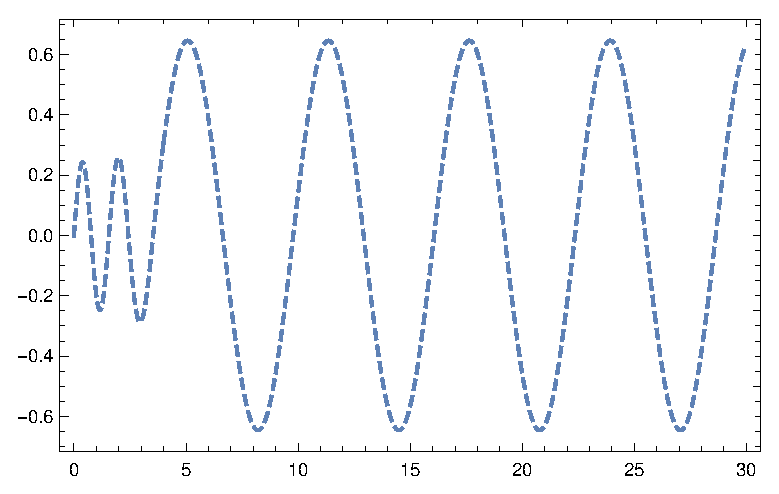
\includegraphics[width=0.42\textwidth]{Scattering.eps}%
\label{fig:b}%
}%
 \caption{\label{TRHO-Figure} (a) The truncated radial harmonic oscillator (solid line) for $b=4$ and their corresponding bound states (dashed lines). (b) The corresponding scattering state for $k=1$.}
\end{figure}

%\begin{figure}
%\begin{center}
%\includegraphics{TRHO-Figure.eps}
%\end{center}
%\caption{\label{TRHO-Figure} The truncated radial harmonic oscillator (dashed line) for $b=4$ and their corresponding bound states (solid lines).}
%\end{figure}

%%%%%%%%%%%%%%%%%%%%%%%%%%%%%%%%%%%%%%%%%%%%%%%%%%%%%%%%%%%%%%%%%%%%%%%%%%%%%%%%%
\subsection{Scattering states.}
%%%%%%%%%%%%%%%%%%%%%%%%%%%%%%%%%%%%%%%%%%%%%%%%%%%%%%%%%%%%%%%%%%%%%%%%%%%%%%%%%

In this case, let us restrict the energy values to the interval $E>0$ in (\ref{TRHO-Psi0}) and, after taking the continuity conditions at the cut off point, we obtain the expression for the scattering solution:

\begin{eqnarray}
\psi_E(r)=A\left\{
\begin{array}{cc}
 \,\, _1F_1(a,3/2;r^2)\, r\, e^{-r^2/2}, & r\leq b  \\[0.2cm]
D(E,b)\, e^{ikr}+ D^{*}(E,b)\, e^{-ikr},&b<r   \label{TRHO-PsiS}
\end{array}
\right.
\end{eqnarray}
where,
\begin{eqnarray*}
D(k)=\frac{A}{6k}e^{-\frac{1}{2}b(b+2ik)}\left\{ 3[i(b^{2}-1)+bk^{2}]\, _1F_1\left(a,\frac{3}{2};b^{2}\right)+ib^{2}(k^{2}+b^{2}-3)\, _1F_1\left(a+1,\frac{5}{2};b^{2}\right)\right\} 
\end{eqnarray*}
The Figure \ref{TRHO-Figure} shows the graphics of a conventional scattering state for a specific value of the energy. As we can see, this kind of solution of the Schr\" odinger equation has an infinity number of zeros and, as we will see, even then it can be used for implementing the degenerated version of the second order Darboux Transformation.

%%%%%%%%%%%%%%%%%%%%%%%%%%%%%%%%%%%%%%%%%%%%%%%%%%%%%%%%%%%%%%%%%%%%%%%%%%%%%%%%%
\section{Darboux deformed truncated harmonic oscillator.}
%%%%%%%%%%%%%%%%%%%%%%%%%%%%%%%%%%%%%%%%%%%%%%%%%%%%%%%%%%%%%%%%%%%%%%%%%%%%%%%%%

In this section, we use a special kind of scattering solution (it behaves as a $sin$ function out of the interaction zone) for implementing a degenerated version of the Darboux transformation, which is given by:

\begin{eqnarray}
\psi_E(r)=\left\{
\begin{array}{cc}
 A_i \,\, _1F_1\left(a_{q},\frac{3}{2};r^{2}\right)re^{-\frac{r^{2}}{2}} , & r\leq b  \\[0.2cm]
A_e\,\sin{[qr+\delta]},&b<r   \label{DDT-TF}
\end{array}
\right.
\end{eqnarray}
where  $A_i$ and $A_e$ are the arbitrary constants in the internal and external regions, respectively; while $a_{q}=\frac{3-q^{2}-b^{2}}{4}$ and $q^{2}=E$. The form of the solution imposed in the external zone leads that the continuity and differentiability of the solution are fulfilled only for some specific values of the parameters  $q=\sqrt{E}$,  $b$ and $\delta$ (see Figure \ref{FigureX}). These values are obtained by the next transcendental algebraic expression:

\begin{eqnarray}
b^{2}\frac{(3+q^{2}-b^{2})}{3}\, _1F_1\left(a_{q}+1,\frac{5}{2};b^{2}\right)-[b^{2}+qb\,\cot{(qb+\delta)}-1]\, _1F_1\left(a,\frac{3}{2};b^{2}\right)=0.\label{ContinuityCondition}
\end{eqnarray}

\begin{figure}
\centering
\subfloat[]{%
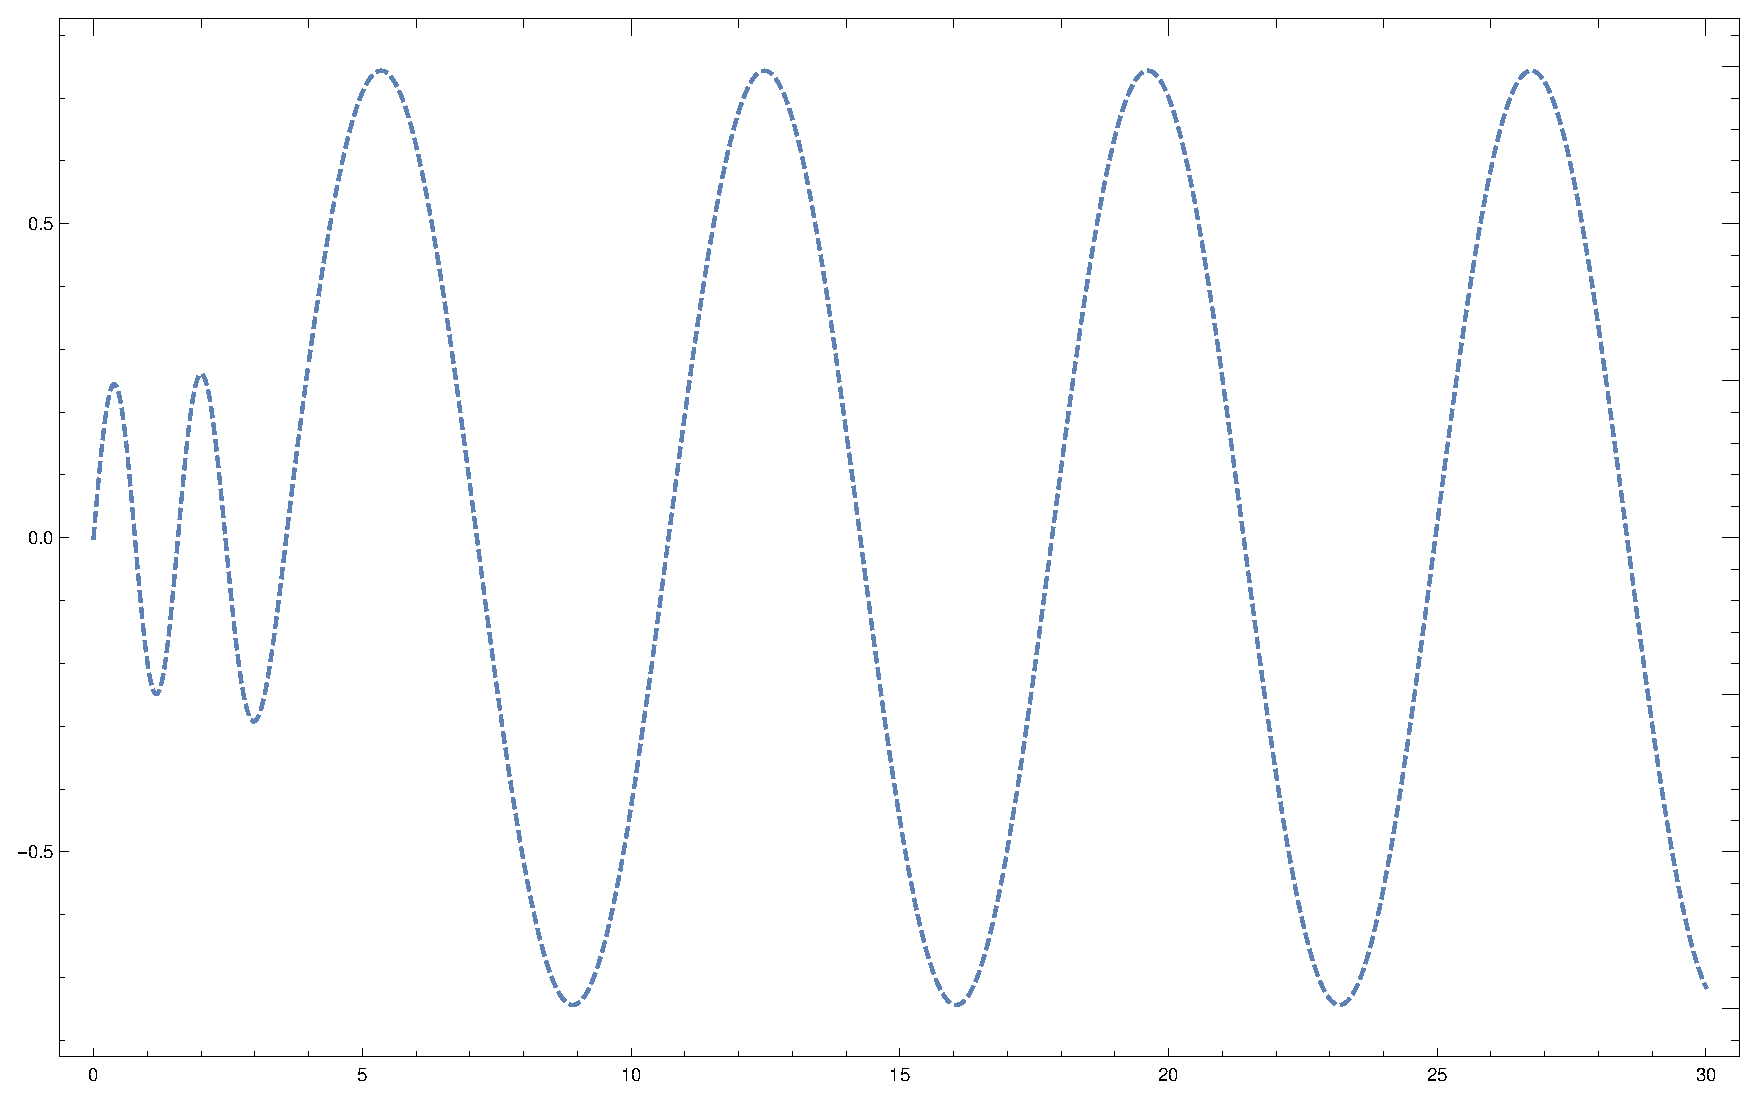
\includegraphics[width=0.41\textwidth]{Differentiable_transformation_function.eps}%
\label{fig:a}%
}%
\hfill%
\subfloat[]{%
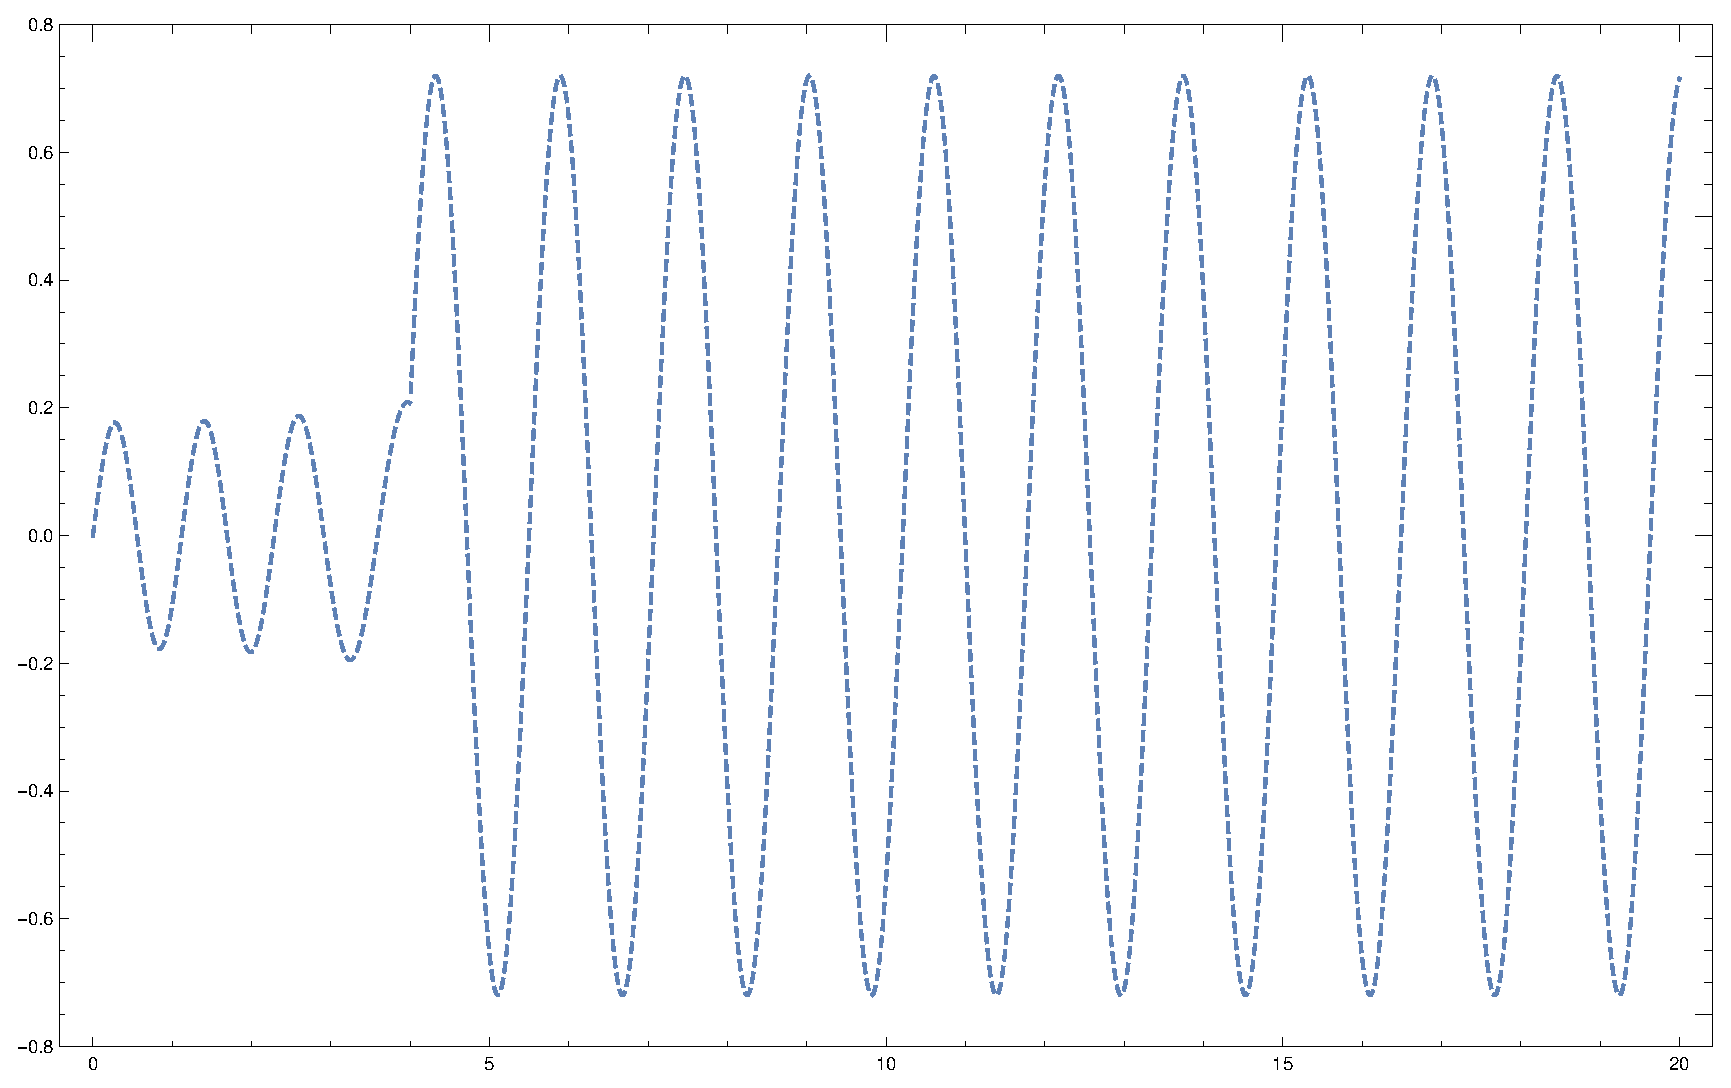
\includegraphics[width=0.41\textwidth]{Not_Differentiable_transformation_function.eps}%
\label{fig:b}%
}%
 \caption{\label{FigureX} (a) Continuous and differentiable scattering state for  the values obtained by solving (\ref{ContinuityCondition}), $b=4$, $\delta =0$ and $q=0.880871$ (b) Non differentiable scattering state at the cut-off point $b=4$,  $\delta =0$ and q=4.}
\end{figure}

However, it is important to mention that the wave functions of the arrival system are not necessarily continuos at the cut-off point, because equation (\ref{vNW-dPsi2}) implies to evaluate second order derivatives of the transformation function. Therefore, to avoid possible discontinuities of the arrival functions, an alternative approach is proposed below.\\

%%%%%%%%%%%%%%%%%%%%%%%%%%%%%%%%%%%%%%%%%%%%%%%%%%%%%%%%%%%%%%%%%%%%%%%%%%%%%%%%%
\subsection{Darboux deformed potential.}
%%%%%%%%%%%%%%%%%%%%%%%%%%%%%%%%%%%%%%%%%%%%%%%%%%%%%%%%%%%%%%%%%%%%%%%%%%%%%%%%%

Since the solution of the initial system is used just as an input for the degenerated Darboux transformation, for the moment we do not should to worry about the continuity of the transformation function, instead we look for the conditions such that the deformed functions are continuous and differentiable. In such a case, we take the next transformation function: 


\begin{eqnarray}
\psi_q(r)=\left\{
\begin{array}{cc}
  _1F_1\left(a_{q},\frac{3}{2};r^{2}\right)re^{-\frac{r^{2}}{2}} , & r\leq b  \\[0.2cm]
\sin{[qr+\delta]},&b<r   \label{DDT-TF1}
\end{array}
\right.
\end{eqnarray}
Here we have omitted the coefficients $A_i$ and $A_e$ due the argument exposed above. Substituting (\ref{DDT-TF1}) into (\ref{vNW-dV2}) we obtain the Darboux deformed potential, whose analytical expression is given by

\begin{eqnarray}
V^{(2)}_{q}(r)=\left\{
\begin{array}{cc}
 V_{<}(r), & r\leq b  \\[0.2cm]
32 q^2\frac{\sin{\theta}-q\,\gamma\,\cos{\theta}}{(\sin{2\theta}-2q\gamma)^2}\sin{\theta},&b<r   \label{DDT-V2}
\end{array}
\right.\end{eqnarray}
where $\theta=qr+\delta$, $\gamma=r+\gamma_0$ and $\gamma_0=\partial_q \delta$.

\begin{equation}
V_{<}=r^{2}-b^{2}-4+\frac{4}{r^2}-2\sum_{n=0}^{\infty}\frac{(a_{q})_{n}\Gamma'(a_{q}+n)}{(3/2)_{n}\Gamma(a_{q}+n)n!}\frac{d^{2}}{dr^{2}}\ln\left\{ \ln {\rm W} \left[  _1F_1\left(a_{q},\frac{3}{2},r^{2}\right),r^{2n}\right]\right\}.\label{DDT-V<}
\end{equation}
Here, $(a_q)_n$ and $\Gamma$ are the factorial and Gamma functions, respectively.  
\begin{figure}
\centering
\subfloat[]{%
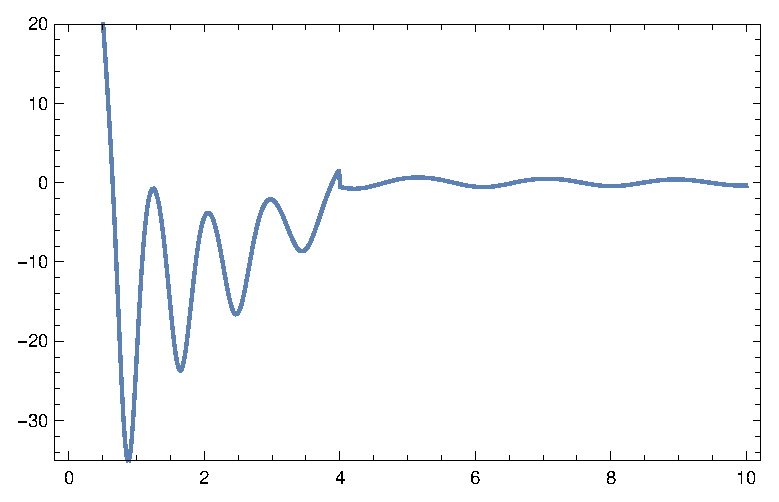
\includegraphics[width=0.41\textwidth]{Potential.eps}%
\label{fig:a}%
}%
\hfill%
\subfloat[]{%
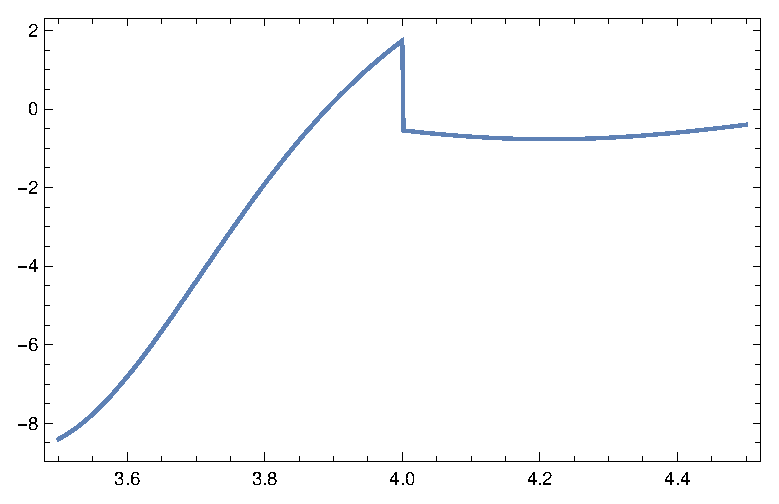
\includegraphics[width=0.41\textwidth]{Potential_discontinuity.eps}%
\label{fig:b}%
}%
\caption{{\label{Figure vNWPot}} (a) Darboux deformed von Neumann Wigner potential for $q=1.65996$ and the next values of the parameters  $b=4$, $\delta=0$ and $\gamma_0=1$. (b) The figure shows a zoom of the discontinuity of the potential at the cut-off point.}
\end{figure}

The Figure (\ref{Figure vNWPot}) shows the plot of  the potential (\ref{DDT-V2}) for some specific parameter values. As we can see, it has an asymptotic divergence at $r=0$, a discontinuity at the cut-off point, an oscillatory behavior and goes to zero as $r$ goes to infinity. Next we explore this last behavior in more detail for $\delta=0$ and $\gamma_0\neq 0$:

\begin{eqnarray*}
\lim_{r\rightarrow\infty} V_q^{(2)}(r)=\lim_{r\rightarrow\infty} 32q^2\frac{[\sin{qr}-q(r+\gamma_0)\cos{qr}]\sin{qr}}{[\sin{2qr}-2q(r+\gamma_0)]^2}\rightarrow -4q\frac{\sin{2qr}}{r}+O\left(\frac{1}{r^2}\right),
\end{eqnarray*}
which is precisely the asymptotic behavior of von Neumann Wigner type potentials, see equation (\ref{vNW-V2}). So, we hope that the potential we have constructed in this section  contains a bound state in the continuum corresponding to the eigenvalue $E=q^2$, which is justly the eigenvalue corresponding to the transformation function.

%%%%%%%%%%%%%%%%%%%%%%%%%%%%%%%%%%%%%%%%%%%%%%%%%%%%%%%%%%%%%%%%%%%%%%%%%%%%%%%%%
\section{Darboux deformed wave functions.}
%%%%%%%%%%%%%%%%%%%%%%%%%%%%%%%%%%%%%%%%%%%%%%%%%%%%%%%%%%%%%%%%%%%%%%%%%%%%%%%%%

As we have proceed for calculating the deformed potential, we will use the expressions (\ref{DDT-TF1})  into (\ref{vNW-dPsi2}) to construct the corresponding solutions of the arrival system, without imposing that the transformation function to be continuous and differentiable, because the boundary conditions will be imposed on the arrival general solution given by: 


\begin{eqnarray}
\psi_k^{(2)}(r)=\left\{
\begin{array}{cc}
 A\psi_{<}(k,r), & r\leq b,  \\[0.2cm]
B F^{+}(k,r)+C F^{-}(k,r),&b<r ,
\end{array}
\right.\label{DDWF}
\end{eqnarray}
where, 
\begin{equation}
\psi_{<}(k,r)=re^{-\frac{r^{2}}{2}}\frac{\sum_{m=0}^{\infty}\frac{(a)_{m}\Gamma'(a_{q}+m)}{(3/2)_{m}\Gamma(a_{q}+m)m!}{\rm W}\left[\, _1F_1\left(a_{q},\frac{3}{2},r^{2}\right),r^{2m},\, _1F_1\left(a,\frac{3}{2},r^{2}\right)\right]}{\sum_{n=0}^{\infty}\frac{(a)_{n}\Gamma'(a_{q}+n)}{(3/2)_{n}\Gamma(a_{q}+n)n!}{\rm W}\left[\, _1F_1\left(a_{q},\frac{3}{2},r^{2}\right),r^{2n}\right]}\label{Psi<}
\end{equation}

\begin{equation}
F^{\pm}(k,r)=\frac{2\gamma q(k^{2}-q^{2})-(k^{2}+q^{2})\mathrm{sin}\,2\theta\pm4ikq\,\mathrm{sin^{2}}\theta}{\mathrm{sin}\,2\theta-2q\gamma}e^{\pm ikr}.\label{PsiPM}
\end{equation}

%%%%%%%%%%%%%%%%%%%%%%%%%%%%%%%%%%%%%%%%%%%%%%%%%%%%%%%%%%%%%%%%%%%%%%%%%%%%%%%%%%%%%%
\subsection{Deformed bound states.}
%%%%%%%%%%%%%%%%%%%%%%%%%%%%%%%%%%%%%%%%%%%%%%%%%%%%%%%%%%%%%%%%%%%%%%%%%%%%%%%%%%%%%%

Now we look for the conventional bond states of the deformed system $E=k^2<0$, then we take $k=i\kappa=i\sqrt{|E|}$. First of all we have to notice that the solution remains regular at the origin of coordinates because $\psi_\kappa(r=0)=0$, while its asymptotic behavior is determined by the functions $F^{\pm}$, whose limit at infinity is given by 

\begin{eqnarray*}
\lim_{r\rightarrow\infty}F^{\pm}(\kappa,r)=-(\kappa^2+q^2)\, e^{\mp \kappa r}.
\end{eqnarray*}

Therefore, to satisfy the square integrable boundary condition we must take $C = 0$ in (\ref{DDWF}). With this in mind and by imposing the continuity of the solution at the cut-off point, we get the bound states of the Darboux deformed system:

\begin{eqnarray}
\psi_{bound}^{(2)}(r)=A\left\{
\begin{array}{cc}
 \psi_{<}^{(2)}(\kappa,r), & r\leq b,  \\[0.2cm]
\frac{ \psi_{<}^{(2)}(\kappa,b)}{F^{+}(\kappa,b)}F^{+}(\kappa,r),&b<r. \label{DD-BoundStates}
\end{array}
\right.
\end{eqnarray} 

\begin{figure}
\begin{center}
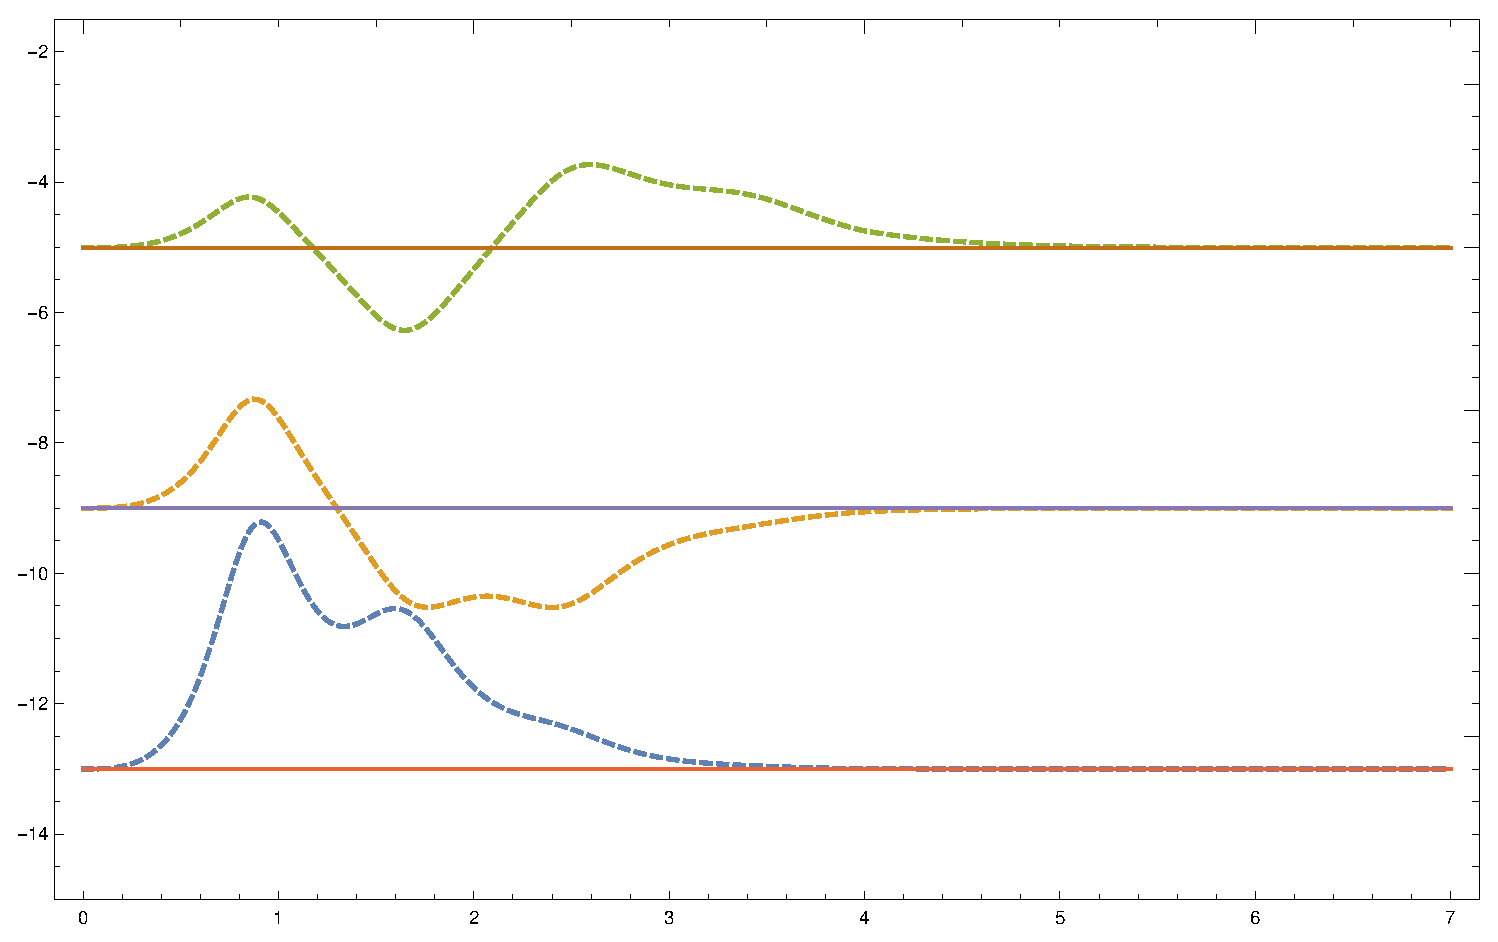
\includegraphics[scale=0.3]{Bound_states.eps}
\end{center}
\caption{\label{DDT-FigBS} The three non normalized bound states corresponding to the discrete spectrum showed in Table 1 and the potential showed in Figure \ref{Figure vNWPot}. The graphs are shown as if the zero of the wave function were in its corresponding eigenvalue.}
\end{figure}

As we can see in Figure \ref{DDT-FigBS}, the bound states of the Darboux deformed potential (Figure \ref{Figure vNWPot})  corresponding to the discrete spectrum showed in Table 1, fulfill the Sturm theorem, that is, the ground state is nodeless while the first and second excited states have one and two zeros, respectively. For the first two states, the maximum amplitude of probability is in the region of greatest depth of the potential, while the maximum amplitude of probability for the most excited state is in the region near the cut-off point.

%%%%%%%%%%%%%%%%%%%%%%%%%%%%%%%%%%%%%%%%%%%%%%%%%%%%%%%%%%%%%%%%%%%%%%%%%%%%%%%%%%%%%%
\subsection{Deformed scattering states.}
%%%%%%%%%%%%%%%%%%%%%%%%%%%%%%%%%%%%%%%%%%%%%%%%%%%%%%%%%%%%%%%%%%%%%%%%%%%%%%%%%%%%%%
Now we explore the continuous regime, that is, the case $E=k^2>0$.  Starting once more  from equation (\ref{DDWF}) and imposing the corresponding continuity conditions at  the cut-off point


\begin{equation}
\begin{array}{c}
\left[B F^{+}(k,r)+C F^{-}(k,r)\right]_{r=b}=[A\psi_{<}(k,r)]_{r=b},\\
\left[B \frac{d}{dr}F^{+}(k,r)+C \frac{d}{dr}F^{-}(k,r)\right]_{r=b}=[A \frac{d}{dr}\psi_{<}(k,r)]_{r=b},
\end{array}
\end{equation}
we get the next relationships between the coefficients 

\begin{eqnarray*}
B=-A \frac{z_{1}^{*}}{z_{2}-z_{2}^{*}},\quad C=A \frac{z_{1}}{z_{2}-z_{2}^{*}},
\end{eqnarray*}
where
\begin{eqnarray*}
z_{1}=\left[\psi_{<}(k,r)\frac{d}{dr}F^{+}(k,r)-F^{+}(k,r)\frac{d}{dr}\psi_{<}(k,r)\right]_{r=b}
\end{eqnarray*}
and
\begin{eqnarray*}
z_{2}=\left[F^{-}(k,r)\frac{d}{dr}F^{+}(k,r)\right]_{r=b}.
\end{eqnarray*}
Here we have used that $\psi_{<}(k,r)$ is a real valued function and $[F^{+}(k,r)]^{*}=F^{-}(k,r)$. Therefore, the scattering solution of the deformed system, for $k\neq q$, can be written as follows:

\begin{eqnarray}
\psi_{s}^{(2)}(r)=A\left\{
\begin{array}{cc}
 \psi_{<}(k,r), & r\leq b,  \\[0.2cm]
\frac{{\rm Im}\left\{\left[ \psi_{<}(k,r)\frac{d}{dr}F^{+}(k,r)-F^{+}(k,r)\frac{d}{dr} \psi_{<}(k,r)\right]_{r=b}F^{-}(k,r)\right\}}{{\rm Im}\left\{\left[F^{-}(k,r)\frac{d}{dr}F^{+}(k,r)\right]_{r=b}\right\}},&b<r, \label{DD-ScatteringStates}
\end{array}
\right.
\end{eqnarray} 
where  ${\rm Im}(z)$ denotes the imaginary part of the complex number $z$. Figure \ref{LastFigure}(a) shows a scattering state of the deformed system for some values of the parameters. Up to this point we have used de degenerated Darboux transformation for constructing the bound and scattering states of the deformed potential showed in Figure (\ref{Figure vNWPot}), which has a von Neumann - Wigner behavior when $r\rightarrow \infty$. Therefore, it is time to examine what happens with the eigenvalue $k=q$ which, according to the asymptotic behavior of the potential, could correspond to a bound state in the continuum.  

\begin{figure}
\centering
\subfloat[]{%
\includegraphics[width=0.41\textwidth]{Scattering_DT.eps}%
\label{fig:a}%
}%
\hfill%
\subfloat[]{%
\includegraphics[width=0.41\textwidth]{BIC.eps}%
\label{fig:b}%
}%
\caption{\label{LastFigure} (a) Scattering state of the Darboux deformed system for k=1, b=4, q=1.65996, $\delta=0$, $\gamma_0=1$. (b) The bound state in the continuum for the eigenvalue $k=q=1.65996$.}
\end{figure}

%%%%%%%%%%%%%%%%%%%%%%%%%%%%%%%%%%%%%%%%%%%%%%%%%%%%%%%%%%%%%%%%%%%%%%%%%%%%%%%%%%%%%%
\section{Existence of a bound state in the continuum.}
%%%%%%%%%%%%%%%%%%%%%%%%%%%%%%%%%%%%%%%%%%%%%%%%%%%%%%%%%%%%%%%%%%%%%%%%%%%%%%%%%%%%%%

The Darboux deformed solutions of the arrival systems are written in terms of the Wronskian whose first entry is precisely the transformation function, equation (\ref{vNW-dPsi2}). Therefore, in this scheme, the scattering solution corresponding to $k=q$ is mapped in principle to the trivial solution. However, since we have the liberty to chose the arbitrary constant 
$A$ in (\ref{DD-ScatteringStates}), we take $A=\frac{A'}{\psi_{<}(k,b)}$, where $A'$ is a new arbitrary constant. In this case, the limit of the solution for $0<r\leq b$, when $k\rightarrow q$, can be evaluated by the L'Hopital rule, that is,   


\begin{equation}
	\lim_{k\rightarrow q}A \psi_{<}(k,r) = A'  \lim_{k\rightarrow q}\frac{\frac{d^2}{dk^2}\psi_{<}(k,r)}{\frac{d^2}{dk^2}\psi_{<}(k,b)}=f(r).
\end{equation}
The explicit form of $f(r)$ is very long and not important at the moment, the only important thing to keep in mind is that $f(r=0)=0$, which guarantees the regularity of the solution at the origin of coordinates. On the other hand, for $r\geq b$, we can to apply again the L'Hopital rule (in this case the rule was applied four times) to obtain the limit of the solution at $k\rightarrow q$, 

\begin{eqnarray*}
&&\lim_{k\to q}\frac{{\rm Im}\left\{\left[\psi_{<}(k,r)\partial_{r}F^{+}(k,r)-F^{+}(k,r)\partial_{r}\psi_{<}(k,r)\right]_{r=b}F^{-}(k,r)\right\}}{\psi_{<}(k,b)[{\rm Im}\left[F^{-}(k,r)\partial_{r}F^{+}(k,r))\right]_{r=b}}  = \frac{f_1(q,b,r)}{f_2(q,b)}.
\end{eqnarray*}
The explicit form of the term $f_2(q,b)$ again is not important,  all we have to keep in mind is that it is different from zero. On the other hand, the term $f_1(q,b,r)$ is given by

\begin{eqnarray*}
f_1(q,b,r)&=& \left[\partial^2_k\psi_{<}(k,r)\partial_r {\rm Re}[F^{+} (k,r)]- \partial^3_{k,k,r}\psi_{<} (k,r){\rm Re}[F^{+}(k,r)]\right]_{k=q,r=b} \,g_1(q,r)\\[0.2cm]
&+&2\left[\partial^2_k\psi_{<}(k,r) \partial^2_{k,r}{\rm Im}\left[F^{+}(k,r)\right] - \partial^2_{k,r}\psi_{<}(k,r)\partial_k {\rm Im} \left[F^{+}(k,r)\right]\right]_{k=q,r=b}\, g_2(q,r)\\[0.2cm]
&+&\frac{2}{\gamma_0}\left[\partial^2_k \psi_{<}(k,r) \partial^2_{k,r}{\rm Re}\left[F^{+}(k,r)\right] - \partial^3_{k,k,r}\psi_{<}(k,r) \partial_k {\rm Re}\left[F^{+}(k,r)\right]\right]_{k=q\,,r=b} \,g_3(q,r)\\[0.2cm]
&+&\left[\partial^3_{k,k,r}\psi_{<}(k,r)\partial^2_k {\rm Im}\left[F^{+}(k,r)\right] - \partial^2_k\psi_{<}(k,r)\partial^3_{k,k,r}{\rm Im}\left[F^{+}(k,r)\right]\right]_{k=q\,,r=b}\, g_3(q,r).
\end{eqnarray*}
Here we have used the notation $\partial_{a_1,...,a_n}^n\equiv \frac{\partial^n}{\partial_{a_1}...\partial_{a_n}}$, while the functions $g_i(q,r)$, are given by

\begin{eqnarray*}
g_1(q,r)&=&\frac{(2 \sin{qr} - 2r ) \sin{[2 (q r + \delta)]} - 
2 q (q r (3 r + 4 \gamma_0) \cos{qr} + 
q r^2 \cos{[2 (q r + \delta)]} + 2 \gamma_0 \sin{qr}}{\sin{2qr}-2q(r+\gamma_0)}\\[0.2cm] 
g_2(q,r)&=& 2q \frac{q(r + 2 \gamma_0) \cos{qr} + qr \cos{[2(qr + \delta)]} - 
2\cos{\delta} \sin{(q r + \delta)}}{-2q(\gamma_0+r)+\sin{[2(qr+\gamma_0)]}},\\[0.2cm] 
g_3(q,r)&=&\frac{2q\sin{(qr + \delta)}}{\sin{[2(qr+\delta)]}-2q(r+\gamma_0)}. 
\end{eqnarray*}

Therefore, 

\begin{eqnarray*}
\lim_{r\rightarrow\infty}g_1(q,r)\rightarrow qr[\cos{qr} + 3 \cos{(qr + \delta)}],\quad
\lim_{r\rightarrow\infty}g_2(q,r)\rightarrow-q[\cos{qr} + \cos{(qr + \delta)}],\quad
\lim_{r\rightarrow\infty}g_3(q,r)\rightarrow0.
\end{eqnarray*}

From the last expressions we can notice that in order to get a square integrable wave function for $k=q$, the coefficients for $g_1(q,r)$ and $g_2(q,r)$ must be simultaneously zero. Taking into account that 

\begin{eqnarray*}\left[{\rm Re}[F^{\pm}(k,r)]\right]_{k=q}=\gamma_0\left[\partial_k{\rm Im}[F^{+}(k,r)]\right]_{k=q}=g_3(q,r),\end{eqnarray*} 
this assumption is true for the values of $q$ that fulfills the next algebraic equation

\begin{equation}
\left[-\partial^2_k\psi_{<}(k,r)\partial_{r}g_3(q,r) + \partial^2_{k,r}\psi_{<}(k,r)g_3(q,r)\right]_{k=q,\,\,r=b}=0.
\end{equation}
This last equation is analogous to the quantization rule of conventional bound states. In the sense that the nature of the deformed interaction region, define the energy for which the bound state in the continuum appears. In this case for $b=4$, $\delta=0$ and $\gamma_0=1$, the bound state in the continuum appears for a value of $q=1.65996$. Figure \ref{LastFigure} shows the graphics of this peculiar state. As we can see it goes to zero as $r\rightarrow\infty$. The physical interpretation of these results underlies that a phenomenon of destructive interference is created between the different parts of the dispersed wave and the multiple crests of the potential, with the net effect that the wave amplitude is canceled  for very large values of $r$ and the wave function becomes normalizable.

\section{Concluding remarks.}

Starting from the truncated radial harmonic oscillator and by taking a special scattering solution as transformation function, a degenerated version of the second order Darboux transformation has been used for constructing a von Neumann Wigner potential type. Unlike the method originally proposed by von Neumann and Wigner, in this case we obtain the complete set of solutions: the bound states, the scattering states and a bound state in the continuum that arises from the solution to an algebraic relationship which plays the role of an analogous to the conventional quantization rule. The main ingredients of the method lie in not requiring that the transformation function be continous and differentiable at the cut-off point, but to impose these conditions  in the arrival solutions, as well as the introduction of a seemingly singular term in the definition of the solution for $ k = q $, which at first, by the nature of the transformation, was mapped into the trivial solution.\\[.2cm]



\begin{thebibliography}{9}
\bibitem{vNW} J. von Neumann and E. Wigner 1929 {\it Phys. Z.} {\bf 30}  p 465
\bibitem{Stillinger} F.H. Stillinger and D.R. Herrick 1975 {\it Phys. Rev. A.} {\bf 11} p 446 
\bibitem{Anzor} A. Khelashvili and N. Kiknadze 1996 {\it J. Phys. A: Math. Gen.} {\bf 29} 3209
\bibitem{Stahlhofen} A.A. Stahlhofen 1996 {\it J. Phys. A: Math. Gen.} {\bf 29} L581
\bibitem{Nature} C. Hsu, B. Zhen, A. Stone et al. 2016 {\it Nat Rev Mater} {\bf 1} p 16048
\bibitem{Pappademos} J. Pappademos, U. Sukhatme and A. Pagnamenta 1993 {\it Phys. Rev. A.} {\bf 48} p 3525
\bibitem{Mondragon} D. Lohr, E. Hern\' andez, A. Ja\' uregui and A. Mondrag\' on 2018 {\it Rev. Mex. Fis.} {\bf 64}  464
\bibitem{Nico1} N. Fern\' andez-Garc\' ia, E. Hern\' andez, A. J\' auregui and A. Mondrag\' on 2013 {\it J. Phys. A: Math. Theor.} {\bf 46} p 175302
\bibitem{Nico2} N. Fern\' andez-Garc\' ia, E. Hern\' andez, A. J\' auregui and A. Mondrag\' on 2014 {\it J. Phys: Conf. Series} {\bf 512} p 012023
\bibitem{Capasso}F. Capasso et. al 1992 {\it Nature} {\bf 358} 5656
\bibitem{Witten}E. Witten 1981 {\it Nucl. Phys. B} {\bf 188}  513
\bibitem{Mielnik} B. Mielnik 1984 {\it J. Math. Phys.} {\bf 25}  3387 
\bibitem{Darboux} V.B. Matveev and M.A. Salle 1991 {\it Darboux Transformations and Solitons} (Berlin Hidelberg: Springer- Verlag)
\bibitem{David} D.J. Fern\' andez C and N Fern\' andez - Garc\' ia 2004 {\it AIP Conference Proceedings} {\bf 744} 236 
\bibitem{Oscar} B. Mielnik and O. Rosas-Ortiz 2004 {\it J. Phys. A: Math. Gen.} {\bf 37}  10007
\bibitem{Zurika} Z. Blanco-Garcia, O. Rosas-Ortiz and K. Zelaya 2019 {\it Math. Meth. Appl. Sci.} {\bf 42} 4925 
\bibitem{Nico3} N. Fern\' andez-Garc\' ia and O Rosas-Ortiz 2008 {\it Ann. Phys.} {\bf 323}  p 1397
\bibitem{Springer} V.B. Matveev and M.A. Salle 1991 {\it Darboux Transformations and Solitons Berlin: Springer}
\bibitem{Nico4} N. Fern\' andez-Garc\' ia 2007 {\it Rev. Mex. Fis.} {\bf S 53} p 42
\bibitem{Nico5} D. Bermudez, D.J. Fern\' andez C and N. Fern\' andez-Garc\' ia 2012 {\it Phys. Lett. A} {\bf 376} p 692
\end{thebibliography}








\end{document}





